\chapter{Lexing with regular expression}
\label{chap:lexing_regular_expr}

\section{Importance of Lexing}
    \subsection{Whitespace Handling}
        This chapter will show why lexing is important in addition to parsing. A
        simple example is whitespace (WS) handling. If we look at the grammar we
        have defined before (N, P, S) the expression " 1 + 1 " is not accepted
        because of whitespace. In order to have WS accepted we can use the
        following rule : $S ::= S '+' WS* P | S '-' WS* P | P$  with WS being
        space, $\backslash$t or $\backslash$n but it is not nice and can quickly
        become a mess. A nicer approach would be to define WS as before and to
        define new rules for operators like $PLUS ::= '+' WS*$.
    \subsection{CFG limitation}
        As we have seen before CFG does not allow reserved work like if.
    \subsection{Performances}
        If we don't use lexing, we need to work on each character, using a lexer
        we can build a token tree which can be ~20 smaller. This is especially
        true if there are fixed overheads (combinators). It is typically
        developed as a loop with switch statement. It is simple enough that we
        can write it by hand or even better generate it (regular expressions)!
\section{Lexers with RE}
    The idea is that we want to match a prefix of the (remainder of) input that
    matches the RE. There are two types of RE flavors : 
    \begin{itemize}
        \item Standard (equivalent to regular grammars) : can be matched in
        $\mathcal{O}(n)$ (n=input size)
        \item Language specific (Perl-Compatible Regular Expression) : often in
        $\mathcal{O}(n)$ but some features can make it exponential (even without
        using them). E.g : backreferencing (capture something we have match and
        try to match it again).
    \end{itemize}

    \newpage
    Some experiment on this subject have been made which show the time needed by
    both techniques to match some rules. As we can see on the next figure the
    difference is huge. Note that, the y axes is not the same, with PCRE we're
    speaking in seconds while in the other approach we are on $\mu$s which is
    way smaller!
    \begin{figure}[H]
         \centering
         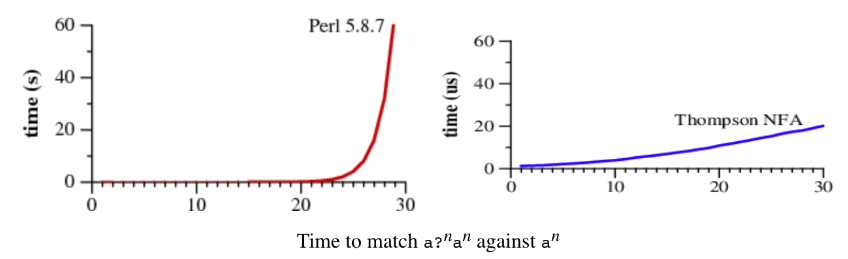
\includegraphics[scale=0.4]{comparison.png}
         \caption{Regular vs PCRE}
         \label{fig:regu_vs_pcre}
    \end{figure}

    However we can ask ourself if this experiment is really realistic. As we
    have seen, it \textit{can} be exponential in some case but are these case
    something that can really happen? This question is not so easy to answer if
    we make some research (Pr. did) we can maybe find one grammar example that
    is both useful and exponential.

    Let's now image that matching a RE is done in $\mathcal{O}(n)$, what is the
    complexity of lexing? It is $\mathcal{O}(n^2)$! Why ? Because in the worst
    case we would need to scan to the end of the input (n) for each token. An
    example would be : $(a | a*x)$ with $a^n$ as input. This is a contrived
    example which is not a problem in practice! This is also a nice example of
    theory vs practice.